% 2011 年陕西卷理科第 3 题：四个函数图象（A 奇函数；B 偶函数且周期 2；C 奇函数；D 偶函数但周期 4）。
% 来源 PDF：普通高考/2011/2011陕西理.pdf，SHA-256 04dab6de0e3ee6223a1cbc126f7f83ae354d2b31201a14db1f31c8477d8a3bed。
% 原页：第 1 页第 1 栏中部，书页码 693。
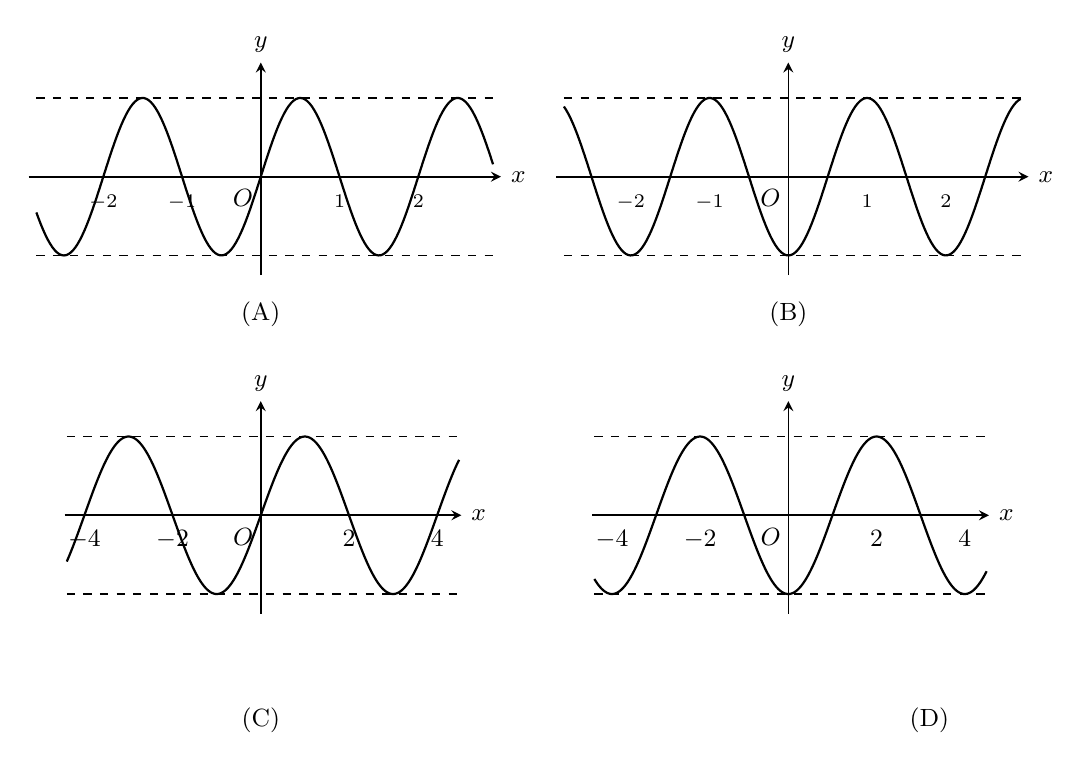
\begin{tikzpicture}[>=stealth, semithick, font=\small]
  % (A) y=sin(pi x)：过原点，奇函数
  \begin{scope}
    \draw[->] (-2.95,0)--(3.05,0) node[right] {$x$};
    \draw[->] (0,-1.25)--(0,1.45) node[above] {$y$};
    \draw[dashed] (-2.85,1)--(2.95,1) (-2.85,-1)--(2.95,-1);
    \draw[thick, domain=-2.85:2.95, samples=200] plot (\x,{sin(180*\x)});
    \foreach \t in {-2,-1,1,2} {\node[below,font=\scriptsize] at (\t,-0.10) {$\t$};}
    \node[below left] at (0.03,-0.04) {$O$};
    \node at (0,-1.75) {(A)};
  \end{scope}
  % (B) y=-cos(pi x)：偶函数，周期 2
  \begin{scope}[xshift=6.7cm]
    \draw[->] (-2.95,0)--(3.05,0) node[right] {$x$};
    \draw[->] (0,-1.25)--(0,1.45) node[above] {$y$};
    \draw[dashed] (-2.85,1)--(2.95,1) (-2.85,-1)--(2.95,-1);
    \draw[thick, domain=-2.85:2.95, samples=200] plot (\x,{-cos(180*\x)});
    \foreach \t in {-2,-1,1,2} {\node[below,font=\scriptsize] at (\t,-0.10) {$\t$};}
    \node[below left] at (0.03,-0.04) {$O$};
    \node at (0,-1.75) {(B)};
  \end{scope}
  % (C) y=sin(pi x/2)：过原点，奇函数
  \begin{scope}[yshift=-4.3cm, xscale=0.56]
    \draw[->] (-4.45,0)--(4.55,0) node[right] {$x$};
    \draw[->] (0,-1.25)--(0,1.45) node[above] {$y$};
    \draw[dashed] (-4.4,1)--(4.5,1) (-4.4,-1)--(4.5,-1);
    \draw[thick, domain=-4.4:4.5, samples=300] plot (\x,{sin(90*\x)});
    \foreach \t in {-4,-2,2,4} {\node[below] at (\t,-0.06) {$\t$};}
    \node[below left] at (0.06,-0.04) {$O$};
    \node at (0,-2.6) {(C)};
  \end{scope}
  % (D) y=-cos(pi x/2)：偶函数，周期 4
  \begin{scope}[yshift=-4.3cm, xshift=6.7cm, xscale=0.56]
    \draw[->] (-4.45,0)--(4.55,0) node[right] {$x$};
    \draw[->] (0,-1.25)--(0,1.45) node[above] {$y$};
    \draw[dashed] (-4.4,1)--(4.5,1) (-4.4,-1)--(4.5,-1);
    \draw[thick, domain=-4.4:4.5, samples=300] plot (\x,{-cos(90*\x)});
    \foreach \t in {-4,-2,2,4} {\node[below] at (\t,-0.06) {$\t$};}
    \node[below left] at (0.06,-0.04) {$O$};
    \node at (3.2,-2.6) {(D)};
  \end{scope}
\end{tikzpicture}
